\RequirePackage{plautopatch}
\documentclass[dvipdfmx,a4paper]{jsarticle}
\usepackage{graphicx}

\usepackage{amsmath}
\usepackage{amssymb}
\usepackage{float}
\usepackage{wrapfig}

\title{船体運動力学 課題 2}
\author{古賀 光一朗}
\date{2025年6月25日}

\begin{document}

    \maketitle
    $$\text{提出期限:2025 年 6 月 30 日(月)10:30AM}$$
    ---
    \begin{wrapfigure}{r}[\dimexpr\marginparsep+\marginparwidth]{0.5\linewidth} % オフセット値を指定
    \centering
    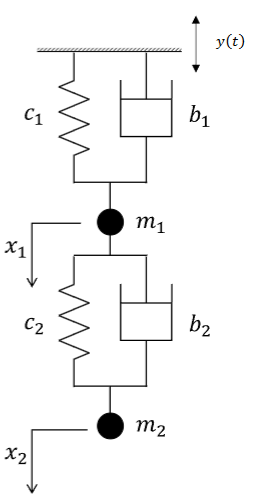
\includegraphics[width=\linewidth]{summer/ship-dynamics/day2_rensei.png}
    \caption{連成したばね-マス-ダッシュポット系}
    \label{fig:damper-system}
    \end{wrapfigure}
右図の連成したばね-マス-ダッシュポット系の支持部(天井)が
\begin{equation}
    y(t)=a\cos{\omega t}
\end{equation}
で定常的に強制動揺されている。なお、システムは線形であり、上下運動しかしない。減衰力は振動減衰を行う程度に小さいとする(過減衰ではない)。


(1-1)質点の無次元化された運動方程式が
\begin{equation}
    \begin{gathered}\ddot{\hat x}+2\Gamma\dot{\hat x}+D\hat x=\Gamma\prime\dot{\hat y}+D\prime\hat y\end{gathered}\\
\end{equation}
で表されるという。このときの$\Gamma, D, \Gamma\prime,D\prime $を数式で示しなさい。
ただし、無次元化は $t=T\hat t , \space x=X\hat x, \space y=X\hat y$ であり、変位ベクトルは次の通りに与える。
$x=\begin{Bmatrix}x_1\\x_2\end{Bmatrix},y=\begin{Bmatrix}y\\0\end{Bmatrix}$


(1-2)固有角周波数の大小による運動の特徴を論じなさい。

\end{document}
